\documentclass[tikz, border=3pt]{standalone}

\usepackage{amsmath,amssymb}
\usepackage{pgfplots}
\pgfplotsset{compat=1.18}
\usepgfplotslibrary{groupplots}
\usetikzlibrary{arrows.meta}
\usepackage{xcolor}

\definecolor{utnblue}{RGB}{0, 51, 102}
\definecolor{utnred}{RGB}{204, 0, 0}

\begin{document}
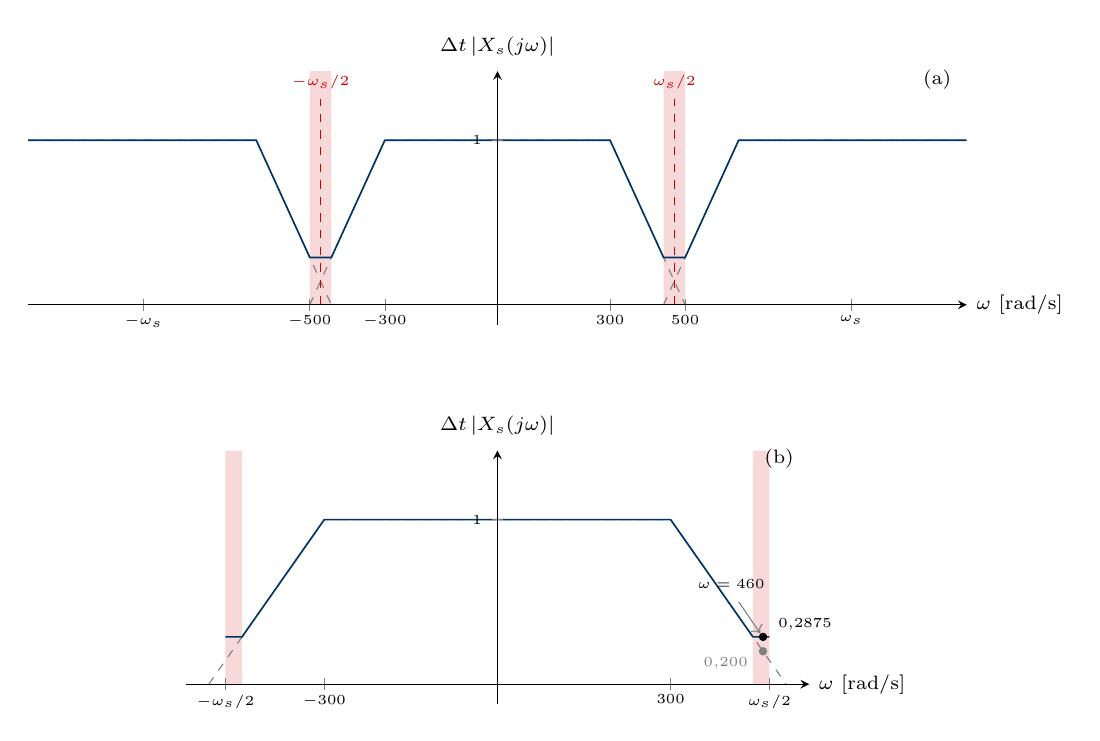
\begin{tikzpicture}[font=\scriptsize]

\begin{groupplot}[
    group style={group size=1 by 2, vertical sep=1.6cm},
    axis lines=middle,
    ymin=-0.12, ymax=1.42,
    tick label style={font=\tiny},
    xticklabel style={fill=white, inner sep=1.5pt},
    label style={font=\scriptsize},
    title style={font=\scriptsize, at={(axis description cs:1,1)},
                 anchor=north east, xshift=-2pt, yshift=-2pt},
    every axis x label/.style={at={(ticklabel* cs:1)}, anchor=west},
    every axis y label/.style={at={(ticklabel* cs:1.02)}, anchor=south},
    xlabel={$\omega$ [rad/s]},
    ylabel={$\Delta t\,|X_s(j\omega)|$},
    enlargelimits=false,
    clip mode=individual,
    axis on top,
]

% =============== (a) copias y solapamiento ===============
\nextgroupplot[title={(a)},
    width=13.5cm, height=4.8cm,
    xmin=-1250, xmax=1250,
    xtick={-942.5,-500,-300,300,500,942.5},
    xticklabels={$-\omega_s$,$-500$,$-300$,$300$,$500$,$\omega_s$},
    ytick={1}, yticklabels={$1$},
]
% zona donde las copias se solapan
\addplot[draw=none, fill=utnred!15]
    coordinates {(442.5,0) (500,0) (500,1.42) (442.5,1.42)} \closedcycle;
\addplot[draw=none, fill=utnred!15]
    coordinates {(-500,0) (-442.5,0) (-442.5,1.42) (-500,1.42)} \closedcycle;

% copias individuales
\addplot[gray, dashed, thin] coordinates {(-500,0) (-300,1) (300,1) (500,0)};
\addplot[gray, dashed, thin] coordinates {(442.5,0) (642.5,1) (1242.5,1) (1250,1)};
\addplot[gray, dashed, thin] coordinates {(-1250,1) (-1242.5,1) (-642.5,1) (-442.5,0)};

% espectro muestreado: suma de las copias
\addplot[utnblue, semithick]
    coordinates {(-1250,1) (-1242.5,1) (-642.5,1) (-500,0.2875) (-442.5,0.2875)
                 (-300,1) (300,1) (442.5,0.2875) (500,0.2875) (642.5,1)
                 (1242.5,1) (1250,1)};

% frecuencia de Nyquist
\addplot[utnred, dashed, thin] coordinates {(471.2,0) (471.2,1.25)};
\addplot[utnred, dashed, thin] coordinates {(-471.2,0) (-471.2,1.25)};
\node[utnred, font=\tiny, anchor=south] at (axis cs:471.2,1.25) {$\omega_s/2$};
\node[utnred, font=\tiny, anchor=south] at (axis cs:-471.2,1.25) {$-\omega_s/2$};

% =============== (b) banda base ===============
\nextgroupplot[title={(b)},
    width=9.5cm, height=4.8cm,
    xmin=-540, xmax=540,
    xtick={-471.2,-300,300,471.2},
    xticklabels={$-\omega_s/2$,$-300$,$300$,$\omega_s/2$},
    ytick={1}, yticklabels={$1$},
]
% zona contaminada de la banda base
\addplot[draw=none, fill=utnred!15]
    coordinates {(442.5,0) (471.2,0) (471.2,1.42) (442.5,1.42)} \closedcycle;
\addplot[draw=none, fill=utnred!15]
    coordinates {(-471.2,0) (-442.5,0) (-442.5,1.42) (-471.2,1.42)} \closedcycle;

% espectro original restringido a la banda base
\addplot[gray, dashed, thin]
    coordinates {(-500,0) (-300,1) (300,1) (500,0)};

% espectro muestreado sobre la banda base
\addplot[utnblue, semithick]
    coordinates {(-471.2,0.2875) (-442.5,0.2875) (-300,1) (300,1) (442.5,0.2875) (471.2,0.2875)};

% componente de 460 rad/s
\addplot[only marks, black, mark=*, mark size=1.3pt] coordinates {(460,0.2875)};
\addplot[only marks, gray,  mark=*, mark size=1.3pt] coordinates {(460,0.200)};
\node[black, font=\tiny, anchor=west, xshift=2pt] at (axis cs:460,0.365) {$0{,}2875$};
\node[gray,  font=\tiny, anchor=east, xshift=-2pt] at (axis cs:460,0.125) {$0{,}200$};
\node[black, font=\tiny, anchor=south] at (axis cs:405,0.52) {$\omega=460$};
\draw[gray, thin, ->] (axis cs:418,0.50) -- (axis cs:455,0.31);

\end{groupplot}

\end{tikzpicture}
\end{document}
